\section{Ejercicio 3}
\subsection{El Problema}
Se tiene una matriz $M$ de tamaño $CxA$. Se tiene una función \texttt{sueldo} que dados un cargo $c_1$ y una antigüedad $a_1$ devuelve un número que se calcula con la siguiente fórmula.

\texttt{sueldo}($c_1$,$a_1$) = $\sum_{i=1}^{c} \sum_{j=1}^{a} M_{i,j}$

Dadas antigüedades $a_1$ y $a_2$ y cargos $c_1$ y $c_2$, se quiere poder calcular la parte de \texttt{sueldo}($a_2$,$c_2$) que jamás podrá ser alcanzada teniendo antigüedad $a_1$ o cargo $c_1$. Se llamará a esta operación \texttt{query} y se calcula con la siguiente fórmula.

\texttt{query}($a_1$,$a_2$,$c_1$,$c_2$) = $\sum_{i=c_1+1}^{c_2} \sum_{j=a_1+1}^{a_2} M_{i,j}$

Dada la matriz y dadas $Q$ queries, se pide implementar un algoritmo que las resuelva con orden de complejidad $O(A*C + Q)$.

\subsection{Desarrollo}

La función \texttt{sueldo} se puede ver como la suma de los elementos de un rectángulo de la matriz $M$. Es el rectángulo de bordes ($1,1$), ($1,a$), ($c,1$) y ($c,a$). Dadas una matriz, cargos $c_1$ y $c_2$ y antigüedades $a_1$ y $a_2$ los rectángulos a sumar para calcular los \texttt{sueldos} correspondientes serían los siguientes:

\begin{figure}[H]
\centering
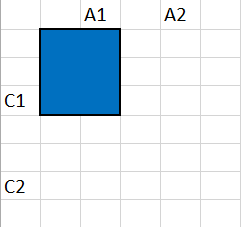
\includegraphics[width=7cm]{Imagenes/Ej3b.png}
\caption{Sueldo con $c_1$ y $a_1$}
\end{figure}

\begin{figure}[H]
\centering
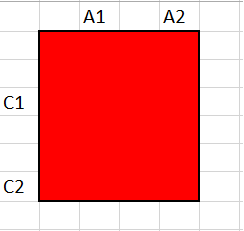
\includegraphics[width=7cm]{Imagenes/Ej3c.png}
\caption{Sueldo con $c_2$ y $a_2$}
\end{figure}

Las queries también pueden verse como suma de elementos de un rectángulo de la matriz. La query para los cargos y antigüedades del ejemplo anterior, se podría ver como la suma de los elementos del rectángulo de bordes ($c_1+1,a_1+1$), ($c_1+1,a_2$), ($c_2,a_1+1$) y ($c_2,a_2$).

\begin{figure}[H]
\centering
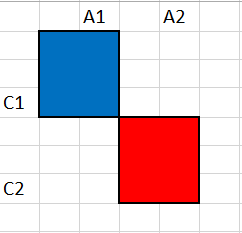
\includegraphics[width=7cm]{Imagenes/Ej3a.png}
\caption{Query con $c_1$, $c_2$, $a_1$ y $a_2$}
\end{figure}

En la figura puede verse en azul el sueldo con cargo $c_1$ y antigüedad $a_1$. En Rojo puede verse la parte que corresponde al sueldo con cargo $c_2$ y antigüedad $a_2$ pero que no puede obtenerse teniendo cargo $c_1$ o antigüedad $a_1$, que es lo que pide la query. Por lo tanto, la suma de los elementos del rectángulo rojo es la respuesta a la query.

Se decidió resolver el problema utilizando una tabla aditiva bidimensional. Sea una tabla aditiva $T$, la idea detrás de la tabla es que en la posición $T_{i,j}$ se encuentra $\sum_{i=1}^{c} \sum_{j=1}^{a} M_{i,j}$ (notar que esto es equivalente a \texttt{sueldo}($c_1,a_1$). Para resolver una query utilizando la tabla, se deben sumar y restar cuatro rectángulos.

La operación a realizar es la siguiente: $T_{c_2,a_2} - T_{c_1,a_2} - T_{c_2,a_1} + T_{c_1,a_1}$. 

En $T_{c_2,a_2}$ se encuentra el sueldo al que se aspira. Sería el rectángulo rojo de la figura del sueldo de $c_2$, $a_2$. Al sumar ese rectángulo se están sumando elementos de más. Por lo tanto, se proceden a restar otros dos rectángulos. Estos son  $T_{c_1,a_2}$ y $T_{c_2,a_1}$ y se pueden observar en las siguientes imagenes.

\begin{figure}[H]
\centering
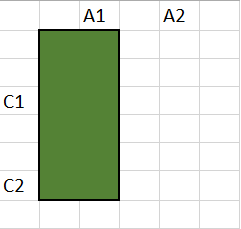
\includegraphics[width=7cm]{Imagenes/Ej3d.png}
\caption{Rectángulo correspondiente a $T_{c_2,a_1}$}
\end{figure}

\begin{figure}[H]
\centering
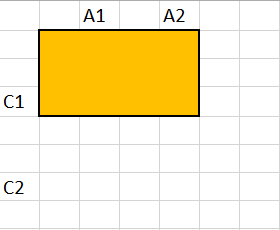
\includegraphics[width=7cm]{Imagenes/Ej3e.png}
\caption{Rectángulo correspondiente a $T_{c_1,a_2}$}
\end{figure}

Una vez restados estos dos rectángulos, se puede ver que el rectángulo correspondiente al sueldo con $c_1,a_1$ (el azul de la primer figura) se restó dos veces, una por cada uno de los dos rectángulos que se restó. Entonces se lo suma una vez. De esta forma lo que queda es el rectángulo rojo de la figura que muestra la resolución de la query. Entonces realizar esa cuenta en la tabla aditiva resuelve la query.

\subsubsection{Implementación}

En esta sección se indexará desde 0. Para implementar la tabla aditiva $T$ se utilizó una matriz de tamaño $(C+1)x(A+1)$. Tanto la primer fila como la primer columna se llenan con ceros. La idea es lograr que valga que para todo elemento de la tabla, $T_{i,j} = \sum_{k=0}^{i-1} \sum_{w=0}^{j-1} M_{k,w}$.

Para armar la tabla, el algoritmo implementado va recorriendo la entrada mientras arma la tabla. Se adjunta un breve pseudocódigo del armado de la tabla.

\begin{verbatim}
for(i in 1..c+1){
    for(j in 1..a+1){
        input(val)
        tabla[i][j] = val + tabla[i-1][j] + tabla[i][j-1] - tabla[i-1][j-1]
    }
}    
\end{verbatim}

En la primera iteración, \texttt{val} $= M_{0,0}$ porque es el primer elemento que se lee. Tras la primera iteración, $T_{1,1} = val$, dado que $T_{1,0} = T_{0,1} = T_{0,0} = 0$. Por lo tanto, $T_{1,1} = M_{0,0} = \sum_{i=0}^{0} \sum_{j=0}^{0} M_{i,j}$.

Luego, en la iteración en la que \texttt{val} $= M_{i,j}$, suponiendo que para cada posición previa de la tabla $T_{a,b} = \sum_{k=0}^{a-1} \sum_{w=0}^{b-1} M_{k,w}$, se quiere ver que al final de la iteración vale que $T_{i+1,j+1} = \sum_{k=0}^{i} \sum_{w=0}^{j} M_{k,w}$.

Se setea $T_{i+1,j+1}$ en \texttt{val} $+ T_{i,j+1} + T_{i+1,j} - T_{i,j}$. Como se ha dicho, \texttt{val} $= M_{i,j}$. Vale que $T_{i,j}$, como es una posición previa de la matriz (porque $i \leq i+1$), contiene la suma $\sum_{k=0}^{i-1} \sum_{w=0}^{j-1} M_{k,w}$. Se pueden ver en la siguiente imagen los rectángulos que representan en la matriz original. En rojo \texttt{val} y en azul $T_{i,j}$.

\begin{figure}[H]
\centering
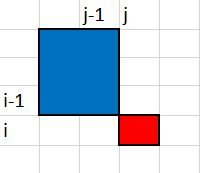
\includegraphics[width=7cm]{Imagenes/Ej3f.png}
\caption{Rectángulo correspondiente a $T_{i,j}$ y \texttt{val}}
\end{figure}

También vale que $T_{i,j+1}$ y $T_{i+1,j}$, como son posiciones previas de la matriz (en el primer caso porque $i \leq i+1$ y en el segundo porque $j \leq j+1$) contienen las sumas correspondientes. Se puede ver en las siguientes imagenes los rectángulos que representan en la matriz original.

\begin{figure}[H]
\centering
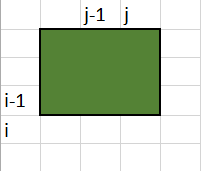
\includegraphics[width=7cm]{Imagenes/Ej3g.png}
\caption{Rectángulo correspondiente a $T_{i,j+1}$}
\end{figure}

\begin{figure}[H]
\centering
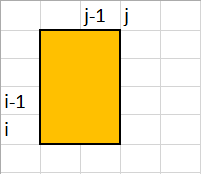
\includegraphics[width=7cm]{Imagenes/Ej3h.png}
\caption{Rectángulo correspondiente a $T_{i+1,j}$}
\end{figure}

Entonces, similarmente al concepto explicado previamente, se puede ver cómo tras la iteración, al sumar los valores de los rectángulos amarillo y verde se está sumando el espacio del azul dos veces. Entonces se resta el azul y al sumarse \texttt{val} se obtiene el rectángulo que se deseaba. Por lo tanto, al terminar la iteración el valor de $T_{i+1,j+1} = \sum_{k=0}^{i} \sum_{w=0}^{j} M_{k,w}$.

\subsubsection{Complejidad}

En esta sección se analizará la complejidad del algoritmo implementado. El algoritmo consiste de dos partes principales.

\begin{itemize}
    \item \textbf{Armado de la Tabla:} Como se analizó en la sección anterior, la tabla se arma mediante un \texttt{for}, recorriendo cada elemento de la matriz de entrada y realizndo una cantidad constante de cuentas por cada uno. Como la cantidad de elementos de la matriz es $A*C$, la complejidad del armado de la tabla es del orden de $O(A*C)$
    \item \textbf{Resolución de Queries:} Luego, por cada una de las $Q$ queries se realiza una cantidad de cuentas constante (la suma explicada con anterioridad). Por lo tanto, se resuelven las queries con complejidad del orden de $O(Q)$.
\end{itemize}

Por lo tanto, la complejidad total del algoritmo es del orden de $O(A*C + Q)$. 

\subsection{Puntaje}
El peso otorgado a este ejercicio es:
